\documentclass[APA,STIX1COL]{WileyNJD-v2}


\usepackage{graphicx}%
\RequirePackage{amsthm,amsmath,mathtools,multirow,amsfonts,bbm,amssymb,xcolor}
\usepackage{mathrsfs}%
\usepackage[title]{appendix}%
\usepackage{textcomp}%
\usepackage{manyfoot}%
\usepackage{booktabs}%
\usepackage{algorithm}%
\usepackage{algorithmicx}%
\usepackage{algpseudocode}%
\usepackage{listings}%
\usepackage{todonotes}
\usepackage{pdflscape}
\usepackage{pdfpages}
\usepackage{setspace} 
\usepackage{longtable}
\usepackage{float}
\hypersetup{
  colorlinks=true,
  citecolor=blue,
  linkcolor=blue,
  urlcolor=blue
}
\usepackage[defaultlines=2,all]{nowidow} % prevent widows and orphans
\usepackage{enumitem} % inline enumeration
\usepackage{subfiles} % for loading supplementary material
\usepackage{changes} % highlight my changes in red
\usepackage[normalem]{ulem} 
\usepackage{cancel}
% \usepackage{subfiles}

\articletype{Article Type}%

\received{\today}
\revised{\today}
\accepted{\today}

\raggedbottom

\begin{document}

\title{This is the sample article title\protect\thanks{This is an example for title footnote.}}

\author[1]{Author One*}

\author[2,3]{Author Two}

\author[3]{Author Three}

\authormark{AUTHOR ONE \textsc{et al}}


\address[1]{\orgdiv{Org Division}, \orgname{Org Name}, \orgaddress{\state{State name}, \country{Country name}}}

\address[2]{\orgdiv{Org Division}, \orgname{Org Name}, \orgaddress{\state{State name}, \country{Country name}}}

\address[3]{\orgdiv{Org Division}, \orgname{Org Name}, \orgaddress{\state{State name}, \country{Country name}}}

\corres{*Corresponding author name, This is sample corresponding address. \email{authorone@gmail.com}}

\presentaddress{This is sample for present address text this is sample for present address text}

\abstract[Summary]{This is sample abstract text this is sample abstract text this is sample abstract text this is sample abstract text this is sample abstract text this is sample abstract text this is sample abstract text this is sample abstract text this is sample abstract text this is sample abstract text this is sample abstract text this is sample abstract text this is sample abstract text this is sample abstract text this is sample abstract text this is sample abstract text this is sample abstract text this is sample abstract text this is sample abstract text this is sample abstract text this is sample abstract text this is sample abstract text this is sample abstract text this is sample abstract text this is sample abstract text this is sample abstract text this is sample abstract text this is sample abstract text.}

\keywords{keyword1, keyword2, keyword3, keyword4}

\jnlcitation{\cname{%
\author{Williams K.}, 
\author{B. Hoskins}, 
\author{R. Lee}, 
\author{G. Masato}, and 
\author{T. Woollings}} (\cyear{2016}), 
\ctitle{A regime analysis of Atlantic winter jet variability applied to evaluate HadGEM3-GC2}, \cjournal{Q.J.R. Meteorol. Soc.}, \cvol{2017;00:1--6}.}

\maketitle

\footnotetext{\textbf{Abbreviations:} ANA, anti-nuclear antibodies; APC, antigen-presenting cells; IRF, interferon regulatory factor}


\section{Introduction}\label{sec:intro}

\section{Methodology}\label{sec:methods}

\section{Simulation Study}\label{sec:sim}

\begin{itemize}
\item We simulate weekly observations for one season at 40 locations over 60 years, with 12 observations per season--year, i.e.\ for a single ``season'', as found in our application section in Section~\ref{sec:app}.
\item At each location \(s\) and year \(t\), the two variables are generated from a bivariate \(t\)-copula with \(\nu=3\) degrees of freedom and known generalized Pareto marginal distributions.
\item The locations are divided into three baseline dependence clusters: \(14\) locations with \(\rho_{s,0}=0.2\), \(13\) with \(\rho_{s,0}=0.5\), and \(13\) with \(\rho_{s,0}=0.8\).

\item A gradual change in the \(t\)-copula correlation parameter is introduced using
\[
\rho_{s,t}
=
\tanh\!\left\{
\operatorname{atanh}(\rho_{s,0})
+
A_s\delta_z g(t)
\right\},
\]
where \(A_s\) indicates whether location \(s\) is affected, \(\delta_z\) controls the magnitude and direction of the change, and \(g(t)\) increases linearly from \(0\) to \(1\) over the specified transition period.

\item The transformation \(\operatorname{atanh}(\rho_{s,0})\) maps the baseline correlation from \((-1,1)\) to the unrestricted real line. The change is applied on this Fisher-\(z\) scale, after which \(\tanh(\cdot)\) maps the linear predictor back to \((-1,1)\), ensuring that the resulting copula correlation remains valid.

\item We consider a local-change setting, in which \(A_s=1\) for only a selected subset of locations, and a global-change setting, in which \(A_s=1\) for all locations.

\end{itemize}

\section{Application to Spanish data}\label{sec:app}

\begin{itemize}
  \item We now apply our changepoint detection algorithm to data from Spain. 
  \item In Section~\ref{subsec:data}, we introduce the dataset of temperatures and precipitation indexes used in our application. 
  \item Section~\ref{subsec:app_screen} shows the results of our initial screening step, while in Section~\ref{subsec:app_cp}, we discuss the results of our changepoint detection algorithm. 
  \item Finally, Section~\ref{subsec:app_clust} shows the clustering results for seasons before and after identified changepoints. 
\end{itemize}

\subsection{Spanish Data}\label{subsec:data}

% \todo{See paper on joint temperature and SPI extremes for rough narrative}
% \begin{itemize}
%   \item We analyse temperature and precipitation data in Spain at 40 sites in mainland Spain (see left panel of Figure~\ref{fig:data}, from 1960 to 2020, inclusive.
%   \item Source of data (ECAD) \todo{Write and reference}
%   \item To aggregate temperature and precipitation into weekly maxes and sums, respectively, which may reduce short-term dependence in the data, as well as reducing the number of zeros observed for precipitation. 
% \end{itemize}
% 
% \begin{itemize}
%   \item We expect there to be a slight lag between temperature and precipitation \todo{word better}
%   \item As such, we turn to using a precipitation index, $\ldots$. 
%   \item \todo{Describe method for precipitation index further}
%   \item By taking a 13-week rolling precipitation index, $\ldots$ \todo{any more info on SPI calculation needed?}
%   \item We also take the negative precipitation index, henceforth  so that we can expect positive extremal dependence with temperature.
% \end{itemize}
% 
% \begin{itemize}
%   \item Describe plot:
%     \begin{itemize}
%       \item As an example, showing temperature vs precipitation index Daroca in Aragon and Jerez De La Frontera in and Andalusia)
%       \item Temperature and ``extreme'' temperature, as defined by its 95th quantile, seems to vary significantly by season for both locations, but only for precipitation index in Jerez De La Frontera \todo{quote 95th quantiles??}
%     \end{itemize}
%   % \item To reduce this marginal temporal dependence, we will consider each season separately 
%   \item To allow for the seasonality present in the marginal data and possibly in the extremal dependence structure, we consider each season separately when modelling dependence and performing our changepoint detection scheme. 
% \end{itemize}
% 
% \begin{figure}[htb]
%     \centering
%     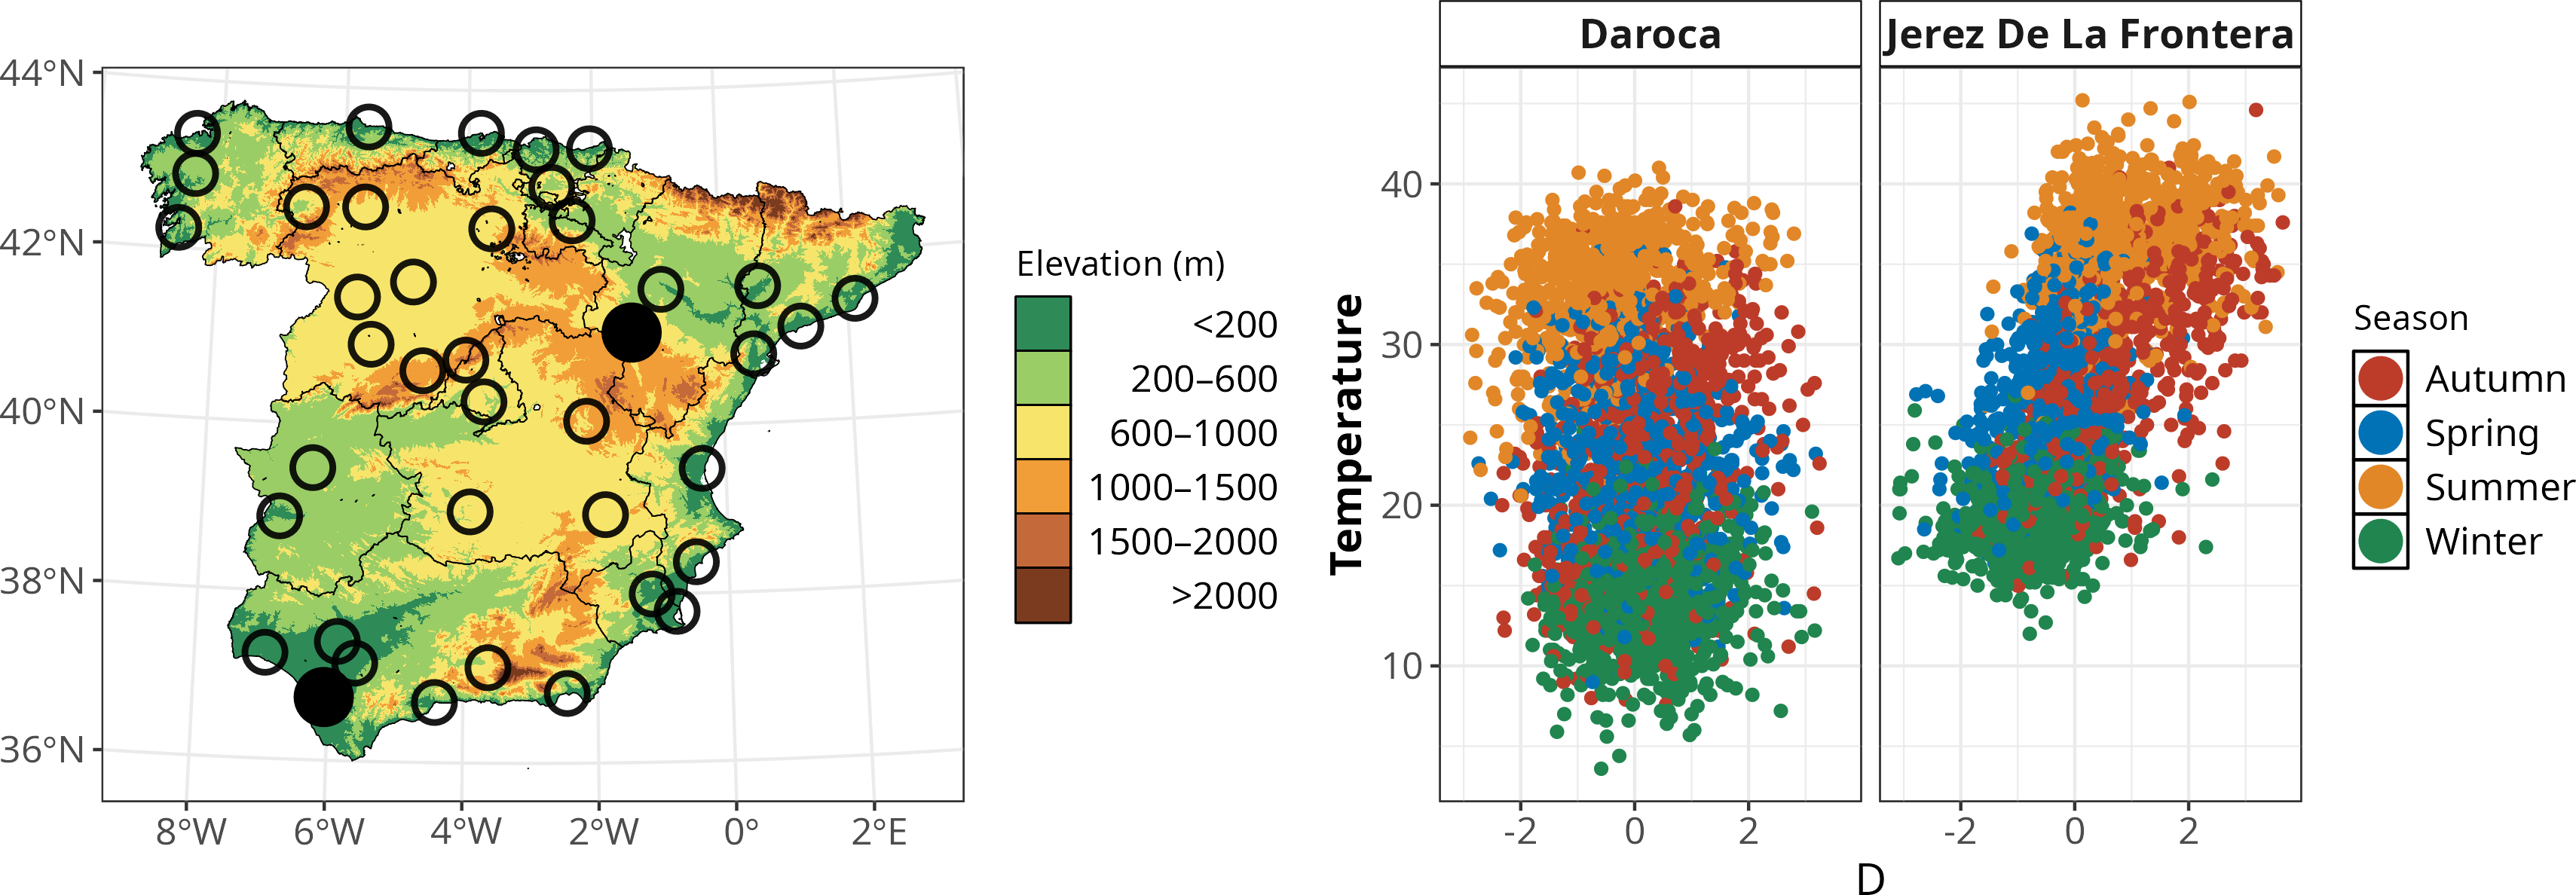
\includegraphics[width = 0.9\linewidth]{plots/intro_trim.png}
%     \caption{
%       Insert here
%     }
%    \label{fig:data}
% \end{figure}

\begin{itemize}
\item We analyse temperature and precipitation observations from 40 meteorological stations distributed across mainland Spain.
\item Their locations are shown in the left panel of Figure~\ref{fig}.
\item The analysis covers the period 1960-2020, inclusive. 
\item Only stations satisfying the required record-length and data-availability criteria are retained. \textcolor{red}{State criteria for choosing stations/locations (description in code)}. 
\item Daily maximum temperature and precipitation totals are obtained from the European Climate Assessment & Dataset (ECA&D) \citep{ECADdaily}. 
\item The ECA&D provides quality-controlled daily meteorological observations from stations across Europe.
\item We aggregate the daily observations to a weekly resolution, taking the maximum recorded temperature and total accumulated precipitation within each week. 
\item This aggregation reduces the influence of very short-range temporal variation and decreases the proportion of zero precipitation observations, although it does not necessarily remove temporal dependence completely.
\end{itemize}

\begin{itemize}
\item The relationship between high temperature and dry conditions may depend more strongly on precipitation accumulated over preceding weeks than on precipitation observed during the same week. 
\item We therefore represent precipitation conditions using the Standardised Precipitation Index (SPI) of \citet{McKee1993}, rather than using weekly precipitation totals directly.
\item At each station, we calculate SPI from precipitation accumulated over a rolling 13-week window. 
\item Thus, the value assigned to a given week summarises precipitation during that week and the preceding 12 weeks, providing a measure of precipitation conditions over an approximately three-month period.
\item The accumulated precipitation is modelled using a Gamma distribution, whose parameters are estimated using unbiased probability-weighted moments. 
\item Its fitted cumulative probability is then transformed to a standard Gaussian scale. 
% \item The calculation is implemented using the \texttt{spi} function from the \texttt{SPEI} package \citep{Begueria2023}, with a rectangular kernel assigning equal weight to each of the 13 weeks.
\item Under the usual SPI convention, negative values represent drier-than-normal conditions and positive values represent wetter-than-normal conditions. 
\item For the dependence analysis, we therefore define the drought index
[
D=-\mathrm{SPI},
]
so that larger values correspond to drier conditions. 
\item This sign convention means that high temperatures and dry conditions are expected to exhibit positive extremal dependence.
\end{itemize}

\begin{itemize}
\item The right-hand panels of Figure~\ref{fig} illustrate the relationship between weekly maximum temperature and the drought index at Daroca, in Aragon, and Jerez de la Frontera, in Andalusia. 
\item These stations are highlighted in the map in the left-hand panel.
\item At both stations, the distribution of weekly maximum temperature differs substantially between seasons. 
\item The seasonal separation in drought-index values is less pronounced at Daroca, whereas Jerez de la Frontera exhibits clearer seasonal variation in both temperature and drought conditions. \textcolor{red}{Mention explicit figures for means/95th quantiles??}
\item These seasonal differences motivate fitting the dependence model and applying the changepoint procedure separately within each season. 
\item This allows both the marginal behaviour and the extremal dependence structure to vary seasonally.
\end{itemize}

\begin{figure}[htb]
\centering
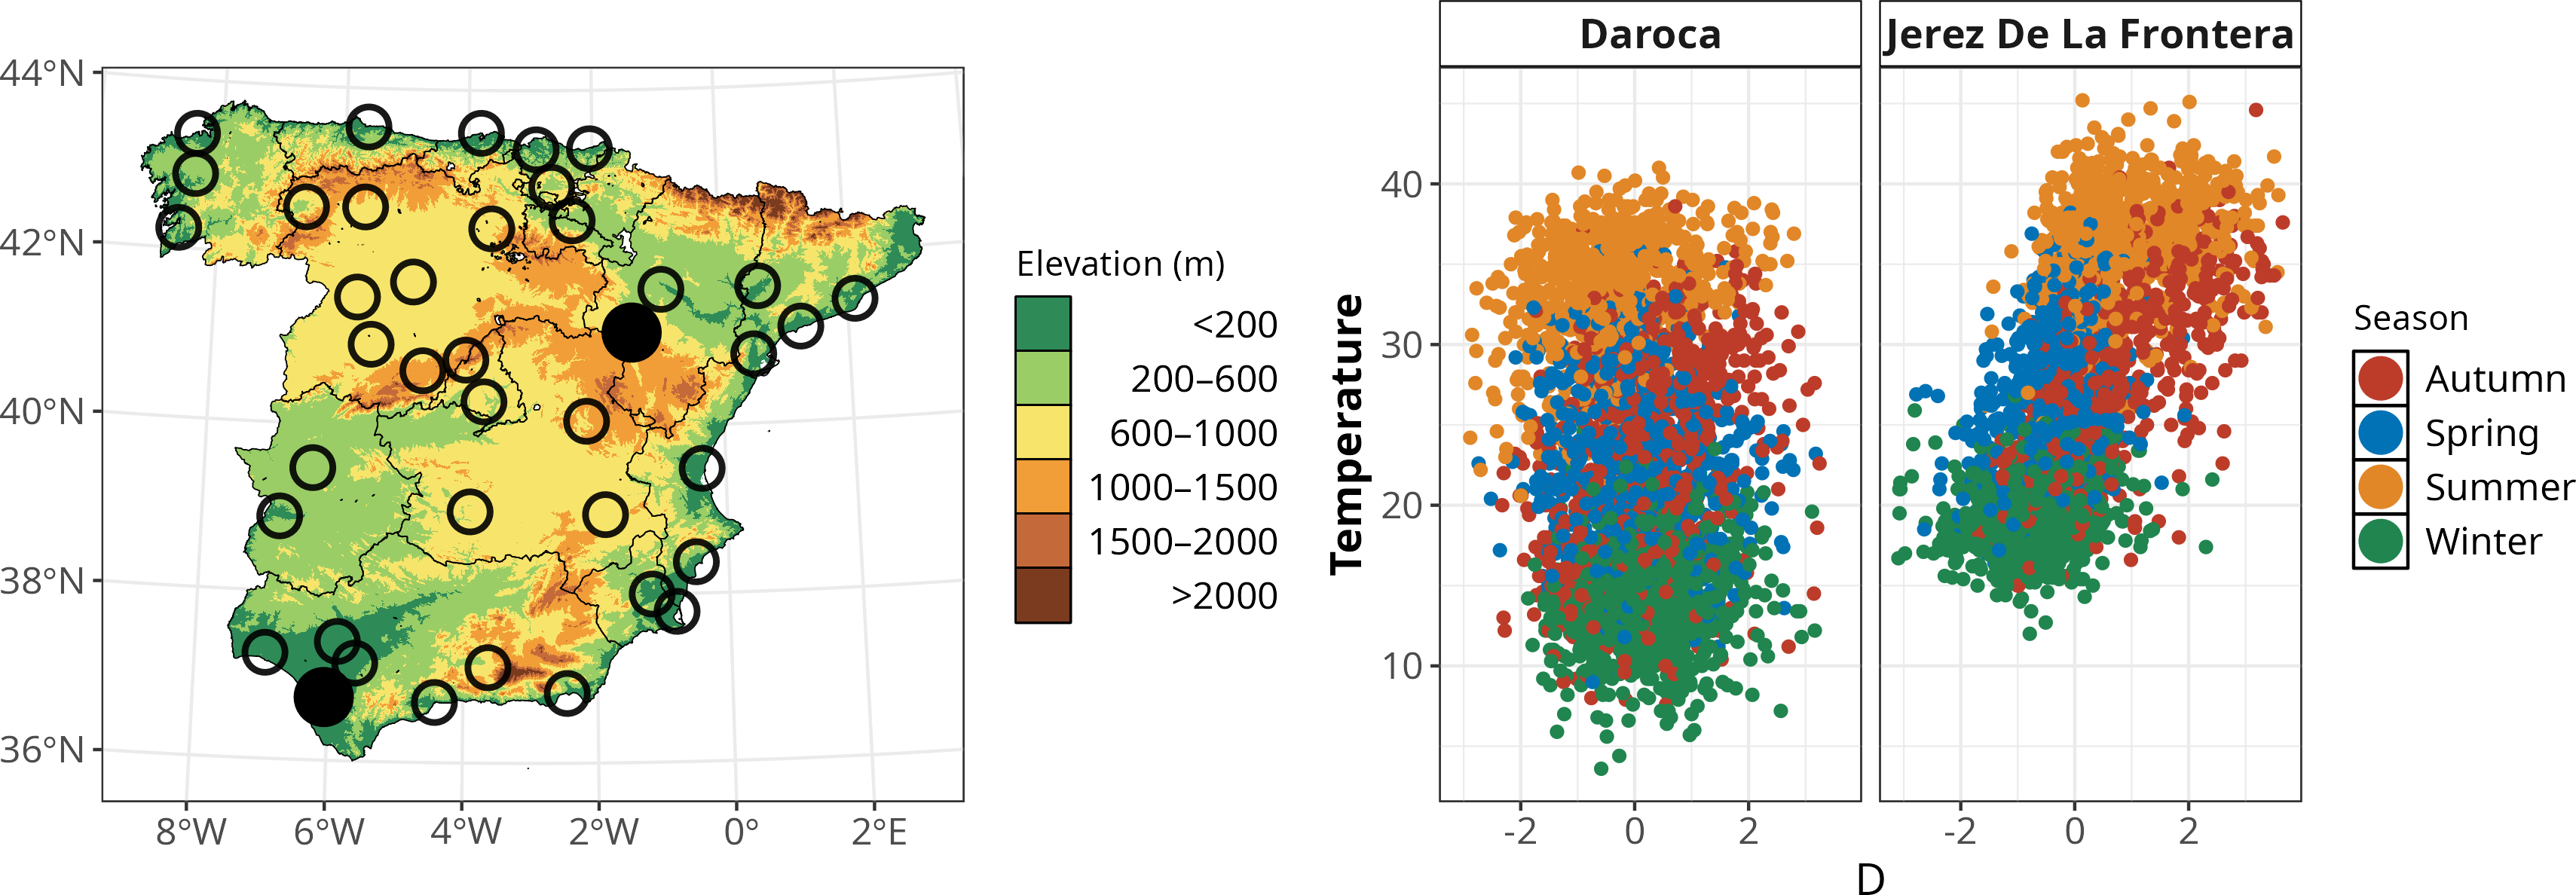
\includegraphics[width=0.9\linewidth]{plots/intro_trim.png}
\caption{
Left: Elevation (m) profile of mainland Spain along with locations of 40 meteorological stations.
Daroca and Jerez de la Frontera highlighted. 
Right: Weekly maximum temperature against 13-week drought index, (D=-\mathrm{SPI}), at these two stations, with observations coloured by season.
}
\label{fig}
\end{figure}

\subsection{Setup}\label{subsec:app_setup}

% % Marginal transformation
% \begin{itemize}
%   \item For both variables, but particularly temperature, there exists some marginal temporal dependence which violates 
%   the assumptions of the conditional extremes model of \citet{Heffernan2007}, namely that of marginal stationarity \todo(Is this correct?)
%   \item Furthermore, there appears to be marginal seasonality present across the year.
%   \item To remove this seasonality, and temporal dependence, we take the data for each individual month across all years, and fit a linear trend by year. 
%   \item By removing this linear trend, we reduce the temporal dependence. 
%   \item Afterwards, we group the data by season, and transform to Laplace margins using the empirical rank transform. 
% \end{itemize}
% 
% % CE
% \begin{itemize}
%   \item For our fitted CE models, we observed good empirical performance, in terms of subsequent clustering solutions exhibiting strong spatial contingency, at the 80th dependence quantile. \todo{Need to do sensitivity analysis}
%   \item All subsequent calculations are also done on the aggregated dissimilarity matrix. \todo{Need to look into others as well}
% \end{itemize}
% 
% % Screening/changepoint setup
% \begin{itemize}
%   \item For our screening step and changepoint detection algorithm, we must perform our permutation test slightly differently to in our simulation study. 
%   \item \todo{Describe how we permutate by `season year', define season year, etc}
%   \item There is an implicit bias-variance tradeoff in the block length used.
%   \item Empirically, we saw good performance with a block length of 25 years, since for a lesser number of years we saw some very large dissimilarities, while 
%     a greater number of years left us with little perspective changepoint timepoints/season years to test at. 
% \end{itemize}

% Marginal preprocessing
\begin{itemize}
\item The conditional extremes framework is applied after transforming each variable to a common marginal distribution. 
\item Consequently, systematic changes in the marginal distributions over time could otherwise be confounded with changes in the extremal dependence structure.
\item Both variables exhibit seasonal variation, while weekly maximum temperature in particular also displays a long-term marginal trend. 
\item We therefore preprocess the marginal distributions before fitting the conditional extremes models.
\item At each station, and for each variable, we consider observations from each calendar month separately and fit a linear trend in year. 
\item The estimated trend is removed from the observations for that month. 
\item Treating months separately allows the magnitude of the temporal trend to vary throughout the year while accounting for the pronounced marginal seasonality.
\item This detrending removes an estimated linear change in the location of each monthly marginal distribution; it does not imply that all temporal dependence has been removed. 
\item In particular, some short-range dependence may remain between successive weekly observations, and consecutive values of the 13-week drought index are constructed from overlapping precipitation windows.
\item Following detrending, the observations are grouped by meteorological season. 
\item For each station and variable, the resulting seasonal observations are transformed standard Laplace margins using the empirical rank transform.
\item The conditional extremes and changepoint analyses are then performed separately for winter, spring, summer and autumn.
\end{itemize}

% Conditional extremes specification
\begin{itemize}
\item We fit the conditional extremes model of \citet{Heffernan2004} using a common dependence threshold equal to the theoretical 80th percentile of the standard Laplace distribution. 
\item The same threshold is used for both variables, at every station, in both temporal blocks and at every candidate changepoint. 
\item This ensures that exceedances have a common interpretation throughout the analysis.
\item The 80th-percentile threshold provided a satisfactory empirical compromise between restricting attention to the joint tail and retaining enough exceedances for stable model estimation. 
\item In particular, the resulting clustering solutions exhibited clear spatial contiguity. \textcolor{red}{Add a sensitivity analysis for the dependence threshold.}
\item The Monte Carlo approximation used to construct the pairwise dissimilarities employs the same sample from the standard Laplace distribution in every temporal comparison. 
\item Holding this sample fixed avoids introducing additional Monte Carlo variation between candidate changepoints.
\item The conditional fits from the two conditioning directions are combined into the aggregated dissimilarity matrix defined in Section~\ref{sec:method}. \textcolor{red}{Test for others}
\item All screening, testing and clustering calculations reported below use this matrix. \textcolor{red}{Confirm terminology and add sensitivity results for the alternative dissimilarity matrices, if required.}
\end{itemize}

% Screening and changepoint-test specification
\begin{itemize}
\item For the Spanish application, the permutation procedure is adapted to preserve the temporal and spatial structure within each season. 
\item Rather than permuting individual weekly observations, we permute complete season-years.
\item For spring, summer and autumn, the season-year is the calendar year in which the observations occur. 
\item Winter spans two calendar years; December is therefore assigned to the same season-year as the following January and February. 
% \item For example, December 1997 and January-February 1998 jointly constitute winter 1998.
\item At a candidate season-year $(t)$, the two temporal blocks consist of the (25) season-years ending at $(t)$ and the (25) season-years beginning at $(t+1)$, respectively. 
\item Thus, $(t)$ denotes a possible change between season-years $(t)$ and $(t+1)$.
\item In each pointwise permutation, the 50 season-years from the two blocks are pooled and randomly divided into two pseudo-blocks containing 25 season-years each. 
\item Every weekly observation belonging to a given season-year is moved as a single unit, and the same reassignment is applied simultaneously to both variables and all 40 stations. 
\item This preserves the dependence between observations within a season-year and the spatial correspondence between stations.
\item The validity of this permutation procedure relies on treating season-years as exchangeable under the null hypothesis of no change in the extremal dependence structure. 
\item Although permuting complete season-years preserves within-year dependence, it does not preserve any residual dependence between successive season-years.
\end{itemize}

% Choice of block length
\begin{itemize}
\item The choice of block length involves a bias-variance trade-off. 
\item Shorter blocks provide better temporal localisation but contain fewer threshold exceedances, resulting in unstable or failed conditional extremes fits. 
\item Longer blocks provide more stable estimates but leave fewer feasible candidate changepoints and smooth changes over a wider temporal interval.
\item We investigated block lengths of 15, 20, 25 and 30 season-years. 
\item With 15-year blocks, many candidate comparisons failed because at least one conditional fit contained too few exceedances. 
\item Twenty-year blocks were reliable for winter but produced substantial failure rates for several other seasons. 
\item All candidate comparisons fitted successfully with 25-year blocks. 
\item Increasing the length to 30 years also produced stable fits, but left only two to five candidate changepoints per season.
\item We therefore use 25 season-years on either side of each candidate throughout the primary analysis. 
\item This was the shortest common block length that produced stable fits across all seasons while retaining a useful range of candidate changepoints. \textcolor{red}{Present the alternative block lengths as a sensitivity analysis or in the supplementary material(?).}
\end{itemize}

\subsection{Screening}\label{subsec:app_screen}

% \todo{Say something about uses of spectral norm, even just for notes}
% % Point of spectral norm: 
% \begin{itemize}
%   \item Figure~\ref{fig:app_screen} shows the results of the screening step for each season for the Frobenius, Infinity and Spectral norms, respectively. \todo{Need for spectral?}
%   \item Several ``peaks'', defined as $\ldots$, are observed across all seasons and choices of norm. \todo{Define how we determine peaks}
%   \item \todo{Describe screening results each season separately (say where peaks are, comment on scale on y-axis and max values)}       
%   \item While this screening step identifies several years of particular interest, there are a sufficiently small number of candidate changepoint years to perform our changepoint algorithm at every timestep.
% \end{itemize}

\begin{itemize}
\item We first perform a computationally less intensive screening step, in which the observed discrepancy between the two estimated dissimilarity matrices is calculated at every feasible candidate season-year without generating a permutation distribution.
\item Figure~\ref{fig:app_screen} presents the screening statistics for each season using the Frobenius, infinity and spectral norms. 
\item As discussed in Section~2, these norms provide complementary summaries of the difference between the dissimilarity matrices on either side of a candidate change.
\item The three norms have different numerical scales, and their absolute values should therefore not be compared directly. 
\item Instead, we compare the timing and relative prominence of features in their respective screening curves.
\item Red points in Figure~\ref{fig:app_screen} identify local peaks. 
\item For a given norm $(T)$, an interior candidate season-year $(t)$ is classified as a local peak when
\[
T(t)>T(t-1)
\qquad\text{and}\qquad
T(t)\geq T(t+1).
\]
The first and final candidate years are not classified as local peaks because they cannot be compared with candidates on both sides.
\end{itemize}

\begin{itemize}
\item For winter, all three norms increase during the late 1990s and exhibit a prominent shared peak in 1998. 
\item A smaller common peak is present around 1992. 
\item The agreement among the norms makes the late-1990s period a particularly notable candidate region.
\item For spring, the clearest screening peak occurs around 1992, for all norms. 
\item Smaller local peaks occur around 1989 and 1997.
\item For summer, the screening curves contain several prominent peaks. 
\item The largest norm values occur in 1988, with further substantial peaks in 1992 and 1997. 
\item For Autumn, the screening results are less concentrated around a single candidate year. 
\item The Frobenius curve has local peaks around 1990 and 1996, while the infinity and spectral curves identify broadly similar candidate regions during the late 1980s or early 1990s and the mid-1990s. 
\item The precise locations of the peaks are less consistent across norms than for winter, spring or summer.
\item Across the four seasons, the largest Frobenius norm screening value occurs for summer around 1988. \textcolor{red}{Cite exact value}
\item The clearest agreement among all three norms occurs around 1992 for spring and around 1998 for winter.
% \item The screening curves identify periods in which the estimated extremal dependence structure differs most strongly between the two temporal blocks, but they do not provide measures of statistical significance. 
% \item Moreover, statistics at neighbouring candidate years are strongly dependent because adjacent 25-year windows share almost all of their observations.
\item Although the screening step highlights several candidate regions of particular interest, the total number of feasible candidate season-years is sufficiently small to apply the permutation test at every candidate. 
\item We therefore retain the complete candidate range rather than restricting the formal analysis to the local screening peaks.
\end{itemize}

\begin{figure}[htb]
\centering
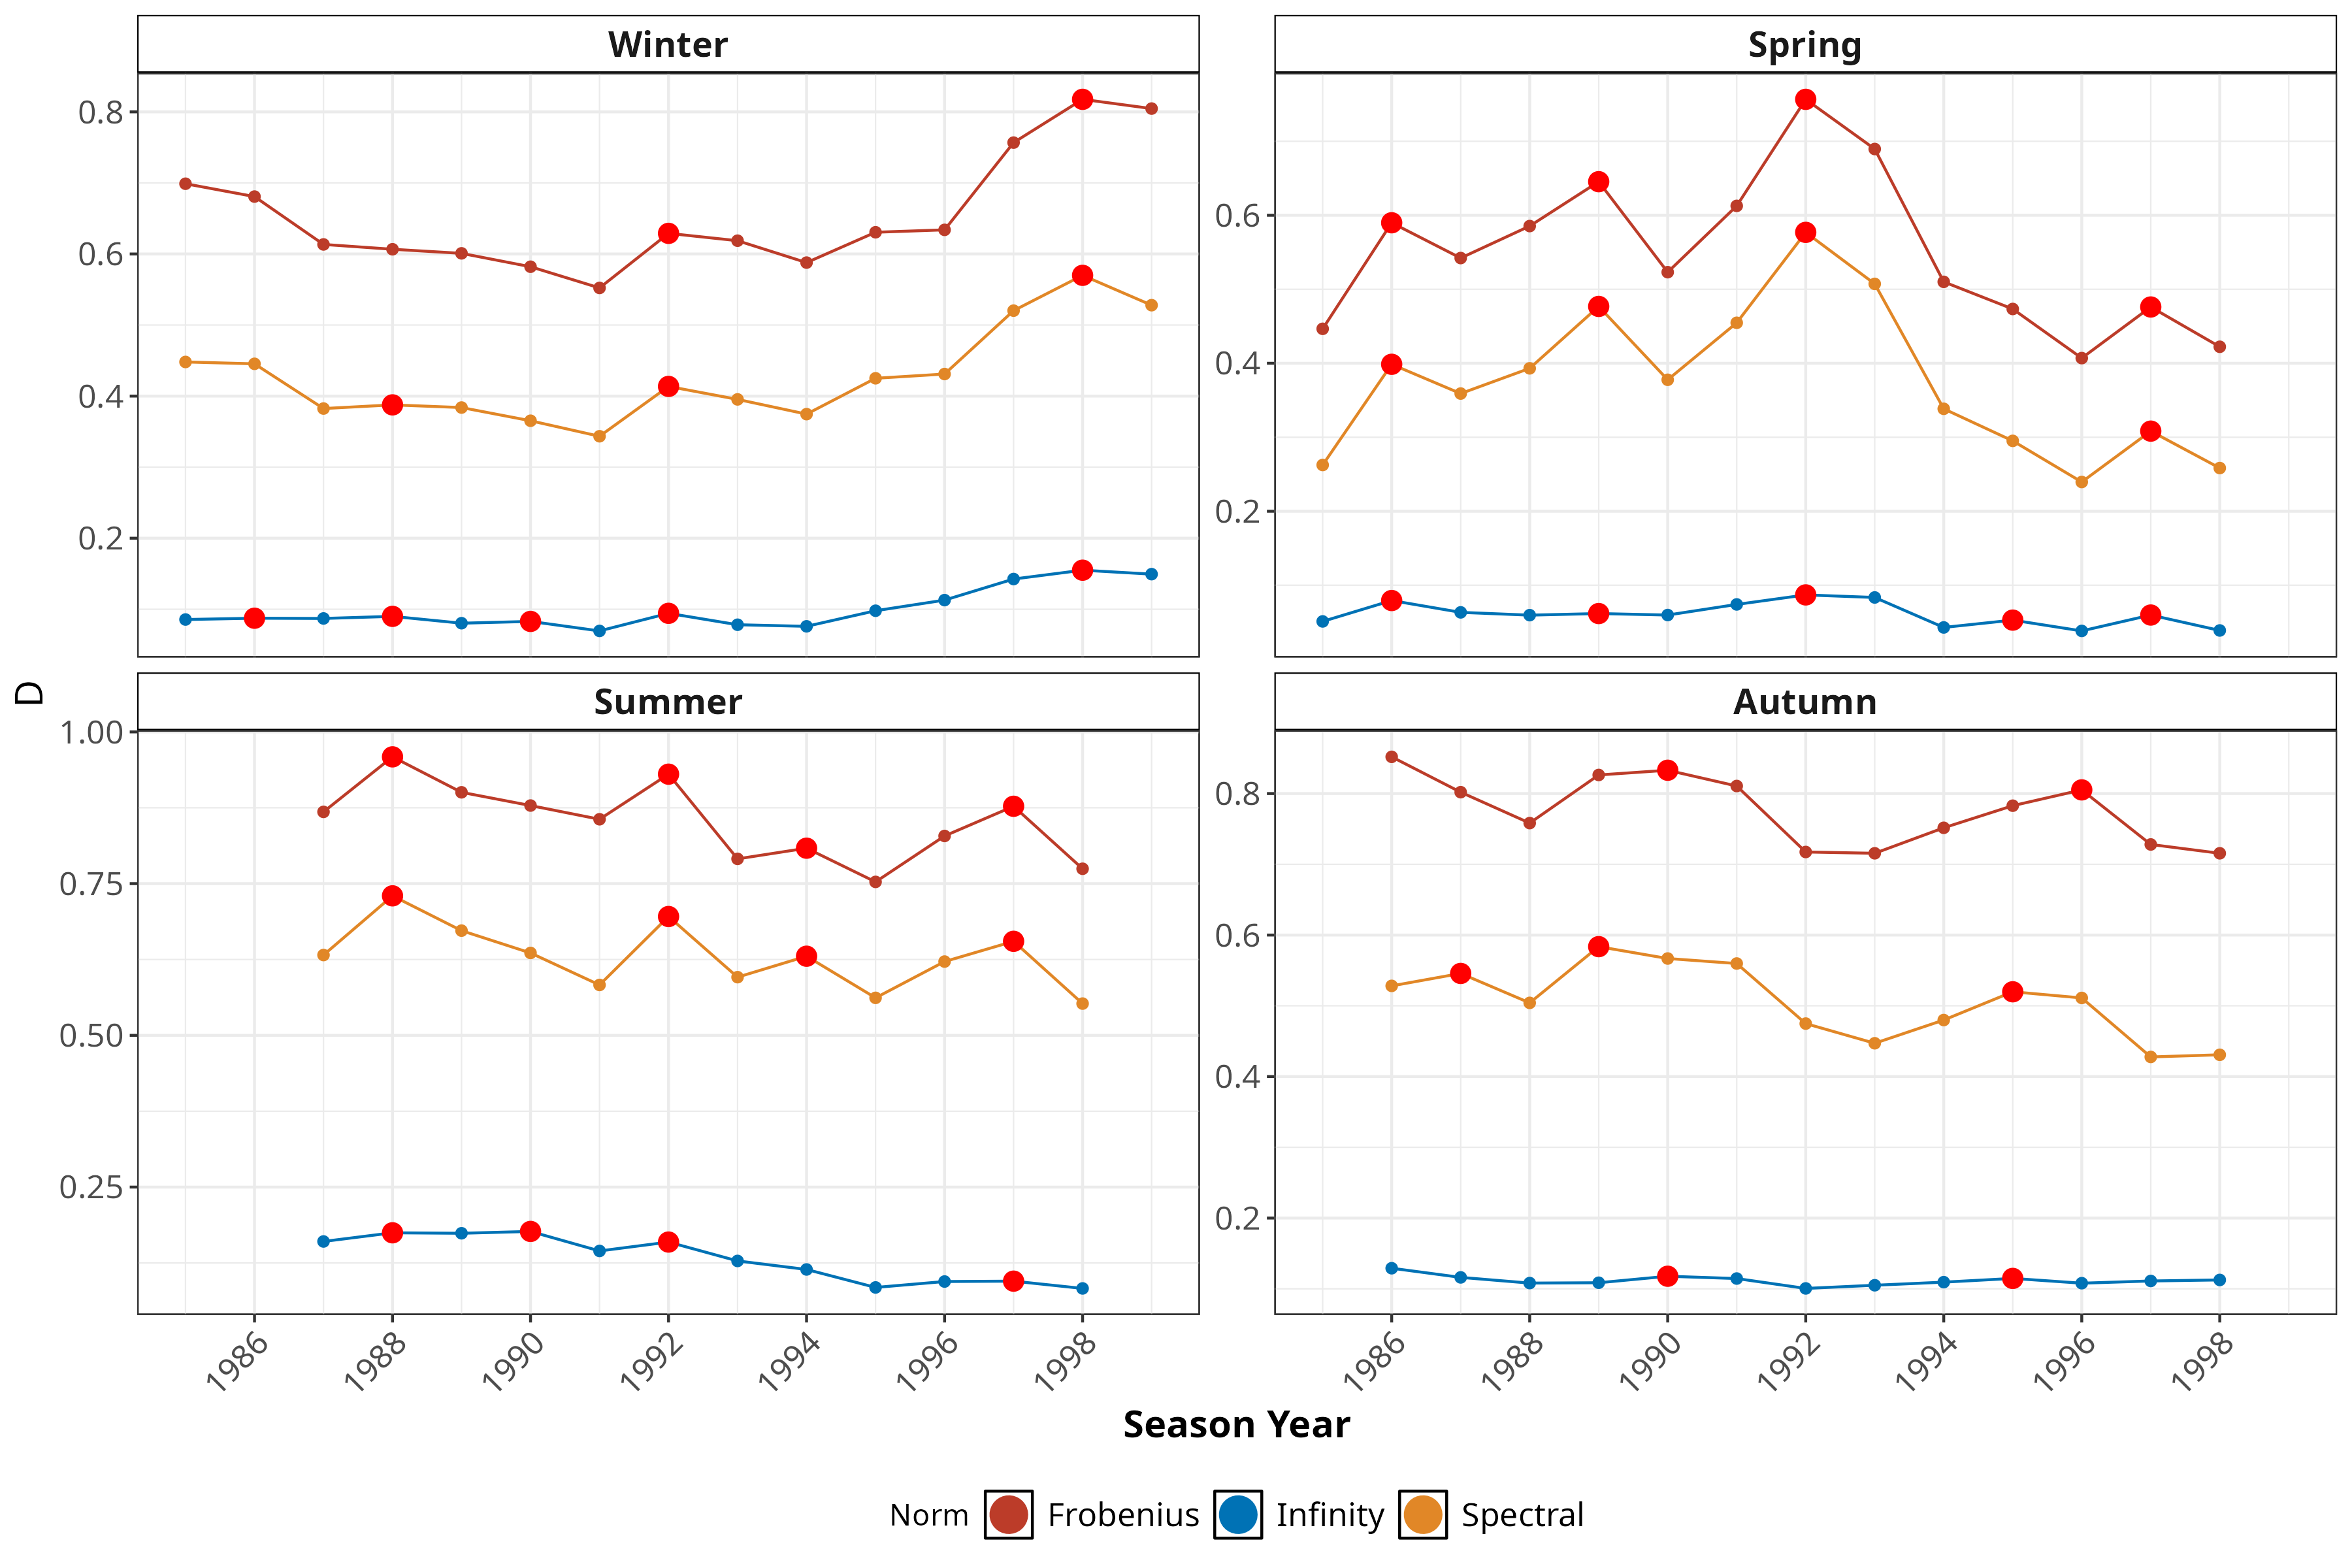
\includegraphics[width=0.9\linewidth]{plots/screen.png}
\caption{
Screening discrepancies between the estimated extremal-dependence dissimilarity matrices on either side of each candidate season-year, calculated using 25 season-years per temporal block. 
Results are shown for the test statistic $D$ using the Frobenius, infinity and spectral norms. 
A candidate $(t)$ represents a possible change between season-years $(t)$ and $(t+1)$. 
Red points denote interior local peaks satisfying $(T(t)>T(t-1))$ and $(T(t)\geq T(t+1))$. 
% Because the three norms have different numerical scales, the timing and relative prominence of their peaks should be compared rather than their absolute magnitudes.
}
\label{fig:app_screen}
\end{figure}

\subsection{Changepoint detection}\label{subsec:app_cp}

% \begin{itemize}
%   \item Figure~\ref{fig:app_cp} shows, for each season, the p-values of the changepoint detection algorithm with 200 permutations at each season year, for each choice of norm. 
%   \item No changepoints are observed for Spring and Autumn at the 5\% significance level, for any season year or norm choice \todo{May have to revise, changepoint is found for Autumn! For now act as if not}
%   \item For Winter, the Infinity norm finds changepoints at the season years from 1996 to 1999, while the other norms find changepoints at 1997 and 1998 only. 
%   \item For Summer, the Infinity norm
%   \item It is interesting that the Infinity norm is most sensitive to the identified changepoints. 
%   \item This may suggest that the changes are sometimes more localised than globally found. 
%   \item Furthermore, for Summer post 1994, the Infinity norm produces the largest p-values, giving extra surety to the conclusion that local changes do not occur around the season years 1994-1998. \todo{Tidy up this conclusion, if even needed/desired!}
%   \item For many of the season years determined to be changepoints for Summer and Winter, the other norm choices also produce significant p-values, and so are in agreement with the Infinity norm. 
% \end{itemize}
% 
% \begin{figure}[htb]
%     \centering
%     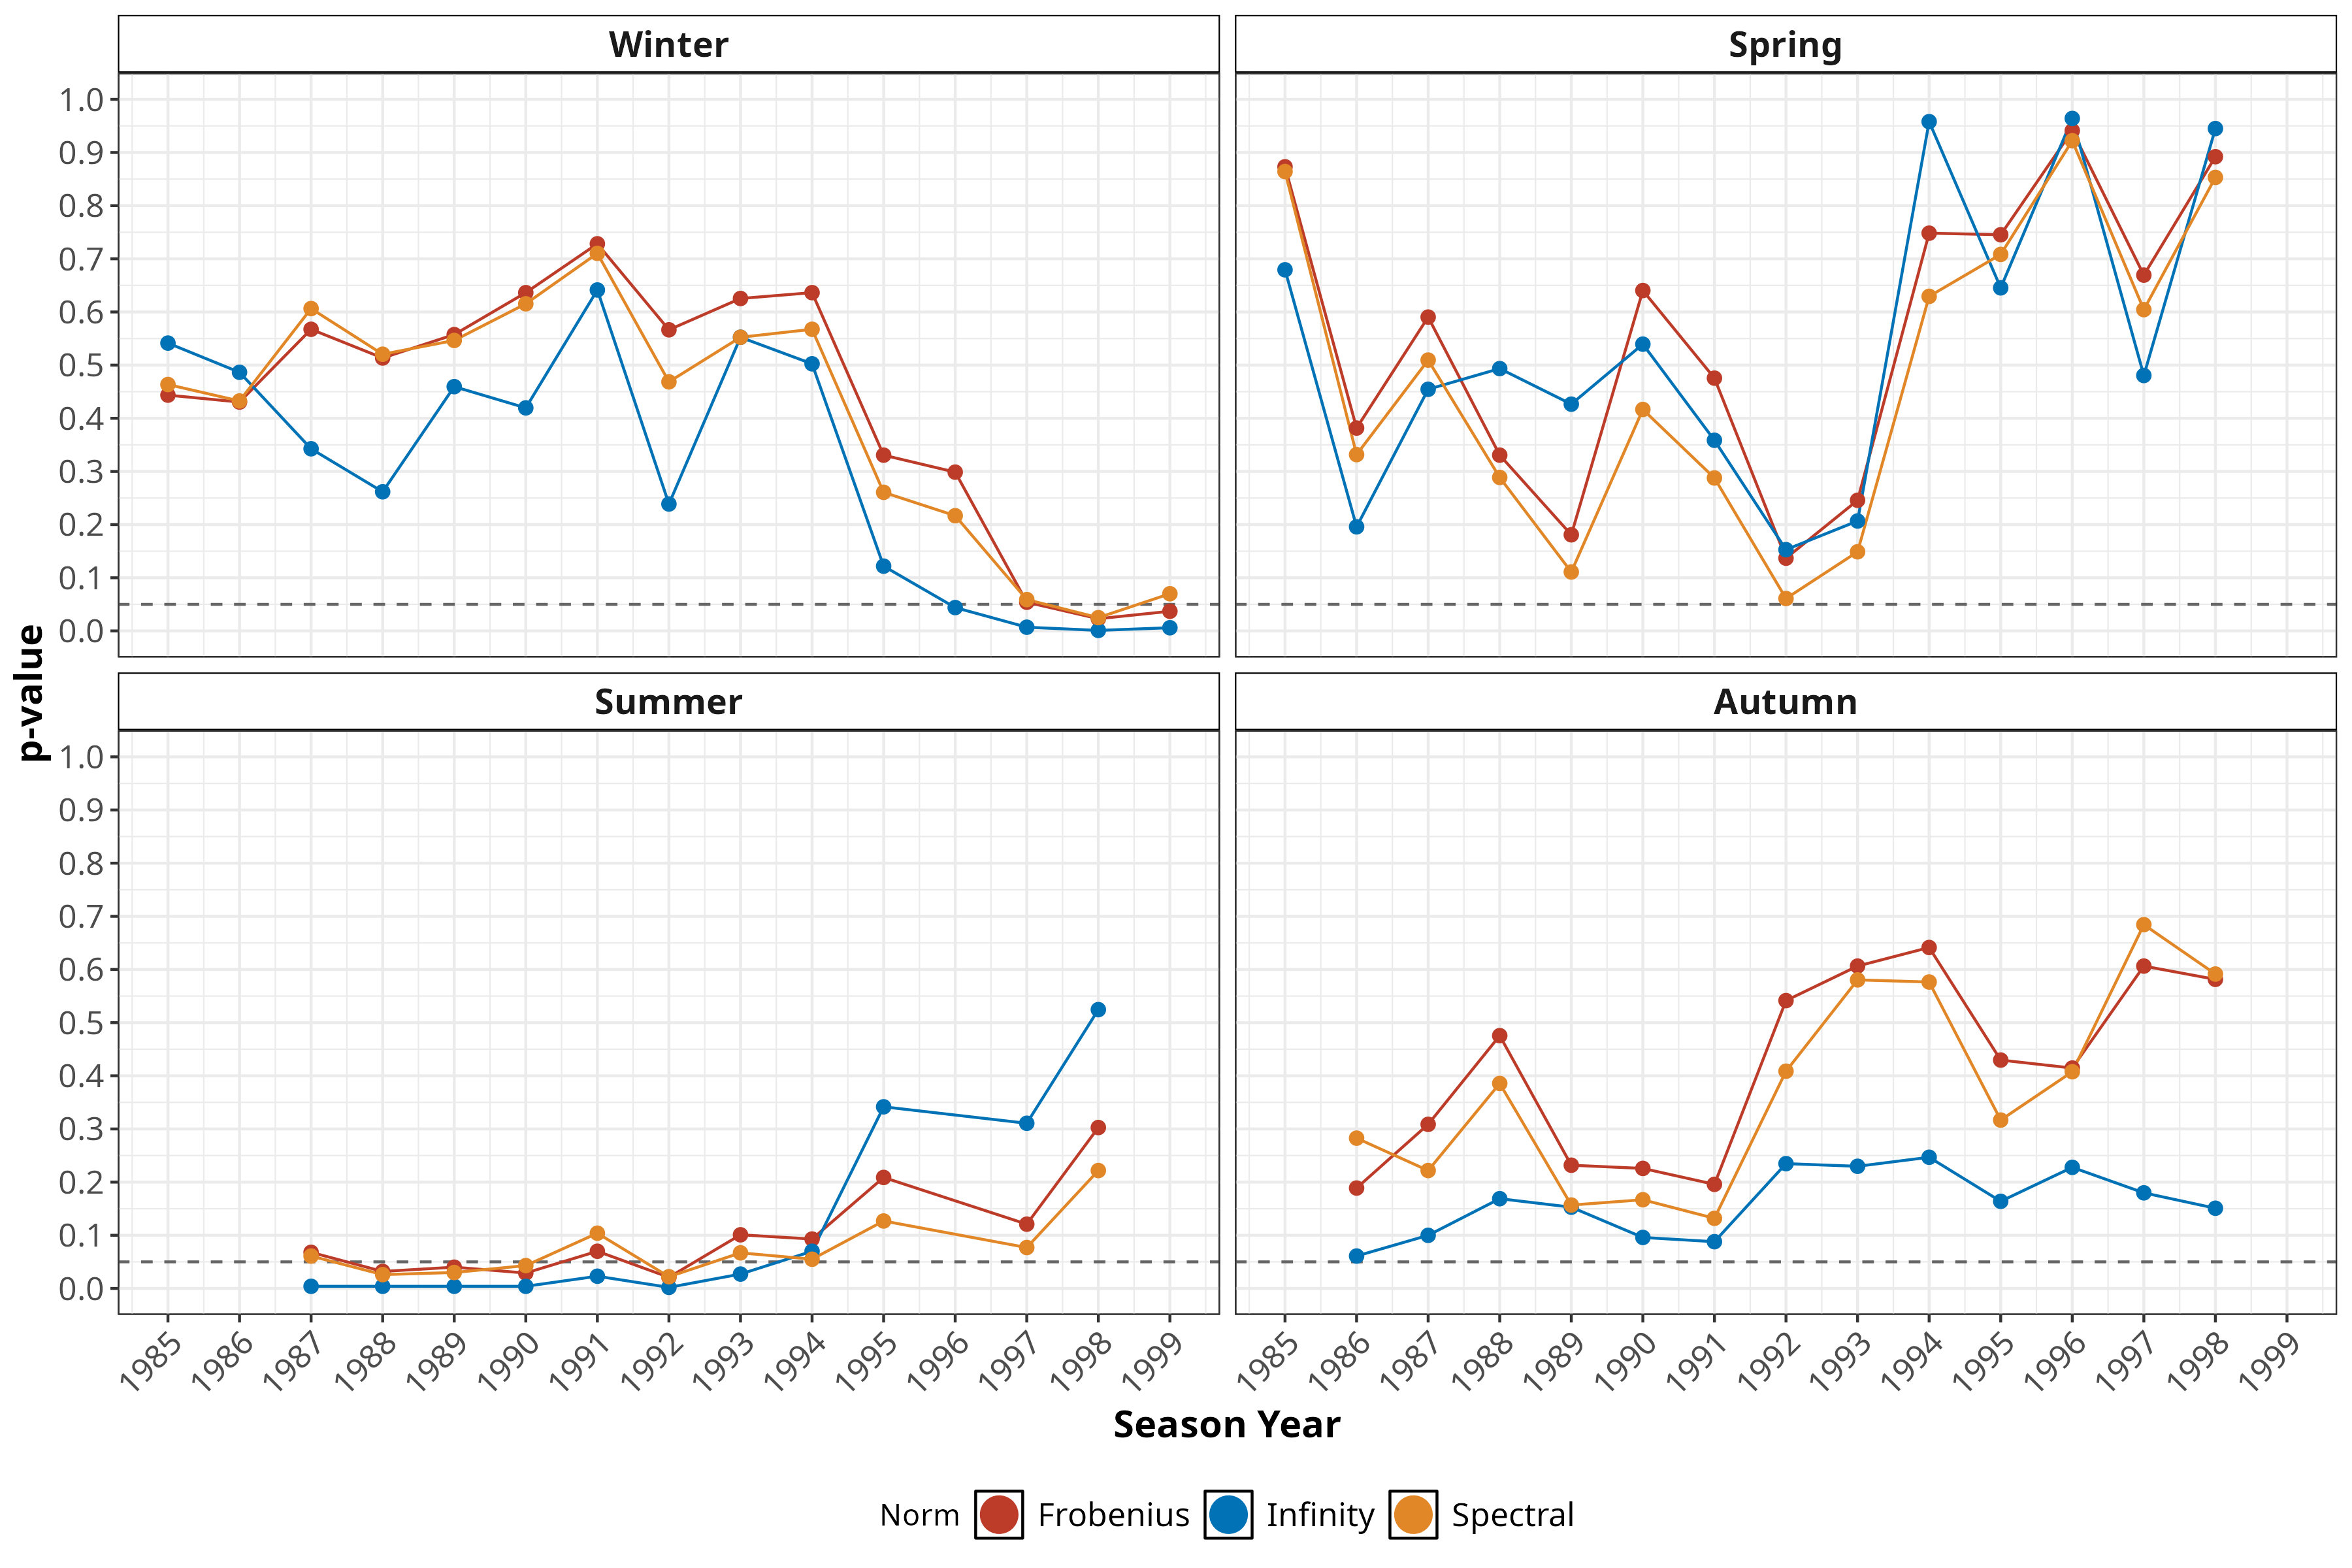
\includegraphics[width = 0.9\linewidth]{plots/change.png}
%     \caption{ 
%       Insert here
%     }
%    \label{fig:app_cp}
% \end{figure}

\begin{itemize}
\item We next apply the permutation test at every feasible candidate season-year. 
\item For each candidate and norm, the null distribution is estimated using 1000 permutations of complete season-years between the two 25-year blocks.
\item Figure~\ref{fig:app_cp} shows the resulting pointwise Monte Carlo p-values for the Frobenius, infinity and spectral norms. 
\item A candidate season-year $(t)$ represents a possible change between season-years $(t)$ and $(t+1)$, and the horizontal dashed line denotes the pointwise 5\% significance level.
\item The p-values in Figure~\ref{fig:app_cp} are pointwise: each tests a change at one specified candidate season-year. 
% \item Because the procedure examines multiple candidate years and three norms, values below 0.05 should initially be interpreted as pointwise evidence rather than as multiplicity-adjusted confirmation of a changepoint. \todo{Replace or supplement these results with Holm-adjusted p-values or a permutation maximum-statistic test for the final analysis.}
\end{itemize}

\begin{itemize}
\item For spring, none of the three norms produces a pointwise p-value below 0.05. 
\item The smallest values occur around 1992, in agreement with the dominant feature identified during screening, but remain above the pointwise significance threshold.

% \item For autumn, the infinity norm produces an isolated pointwise-significant result at the beginning of the candidate range, around 1986. \todo{Add changepoint to re-clustering plot!}
% \item The Frobenius and spectral norms provide no corresponding evidence at this candidate, and no later autumn candidate is significant. 
% \item This isolated result should therefore be interpreted cautiously, particularly because it occurs at the boundary of the candidate range and is not supported by the other norms.
\item Also for Autumn, none of the three norms produces a pointwise p-value below 0.05, although the infinity norm came very close for 1986, the year with the highest test statistic in our screening step. 

\item For winter, the infinity norm provides pointwise evidence of a change over the period 1996--1999. 
\item The spectral norm supports a narrower region around 1997--1998, while the Frobenius norm is significant in 1998. 
\item Thus, all three norms identify 1998, and the overall pattern provides consistent evidence for a change in the winter extremal dependence structure during the late 1990s.

\item For summer, the infinity norm produces pointwise-significant p-values over an extended period from approximately 1987 to 1993. 
\item The Frobenius and spectral norms support narrower subsets of this region, with particularly small p-values around 1988-1990 and 1992.
\item The agreement among the norms indicates that the early-1990s signal is not confined to a single choice of discrepancy statistic.

\item After approximately 1994, the summer p-values generally increase, particularly for the infinity norm.
\item These results provide no pointwise evidence for a change at these later candidates. 
\item However, the relatively large p-values should not be interpreted as affirmative evidence that the dependence structure is unchanged; they indicate only that the observed discrepancies are not unusual under the corresponding permutation null distributions.
\end{itemize}

\begin{itemize}
\item The infinity norm identifies broader pointwise-significant candidate ranges than the Frobenius and spectral norms for both summer and winter. 
\item As discussed in Section~\ref{sec:method}, this may indicate that some changes are more pronounced in particular entries of the dissimilarity matrix than across its entire structure.

\item Nevertheless, the principal summer and winter candidate regions are supported by more than one norm. 
\item In particular, all three norms provide pointwise evidence around 1990 for summer and around 1998 for winter.

\item Taken together, the results suggest candidate changes in the summer extremal dependence structure during the late 1980s or early 1990s and in the winter structure during the late 1990s. 
\item No comparable evidence is found for spring or autumn. % , while the isolated autumn infinity-norm result requires further assessment after accounting for the scan over candidate years.
\end{itemize}

\begin{figure}[htb]
\centering
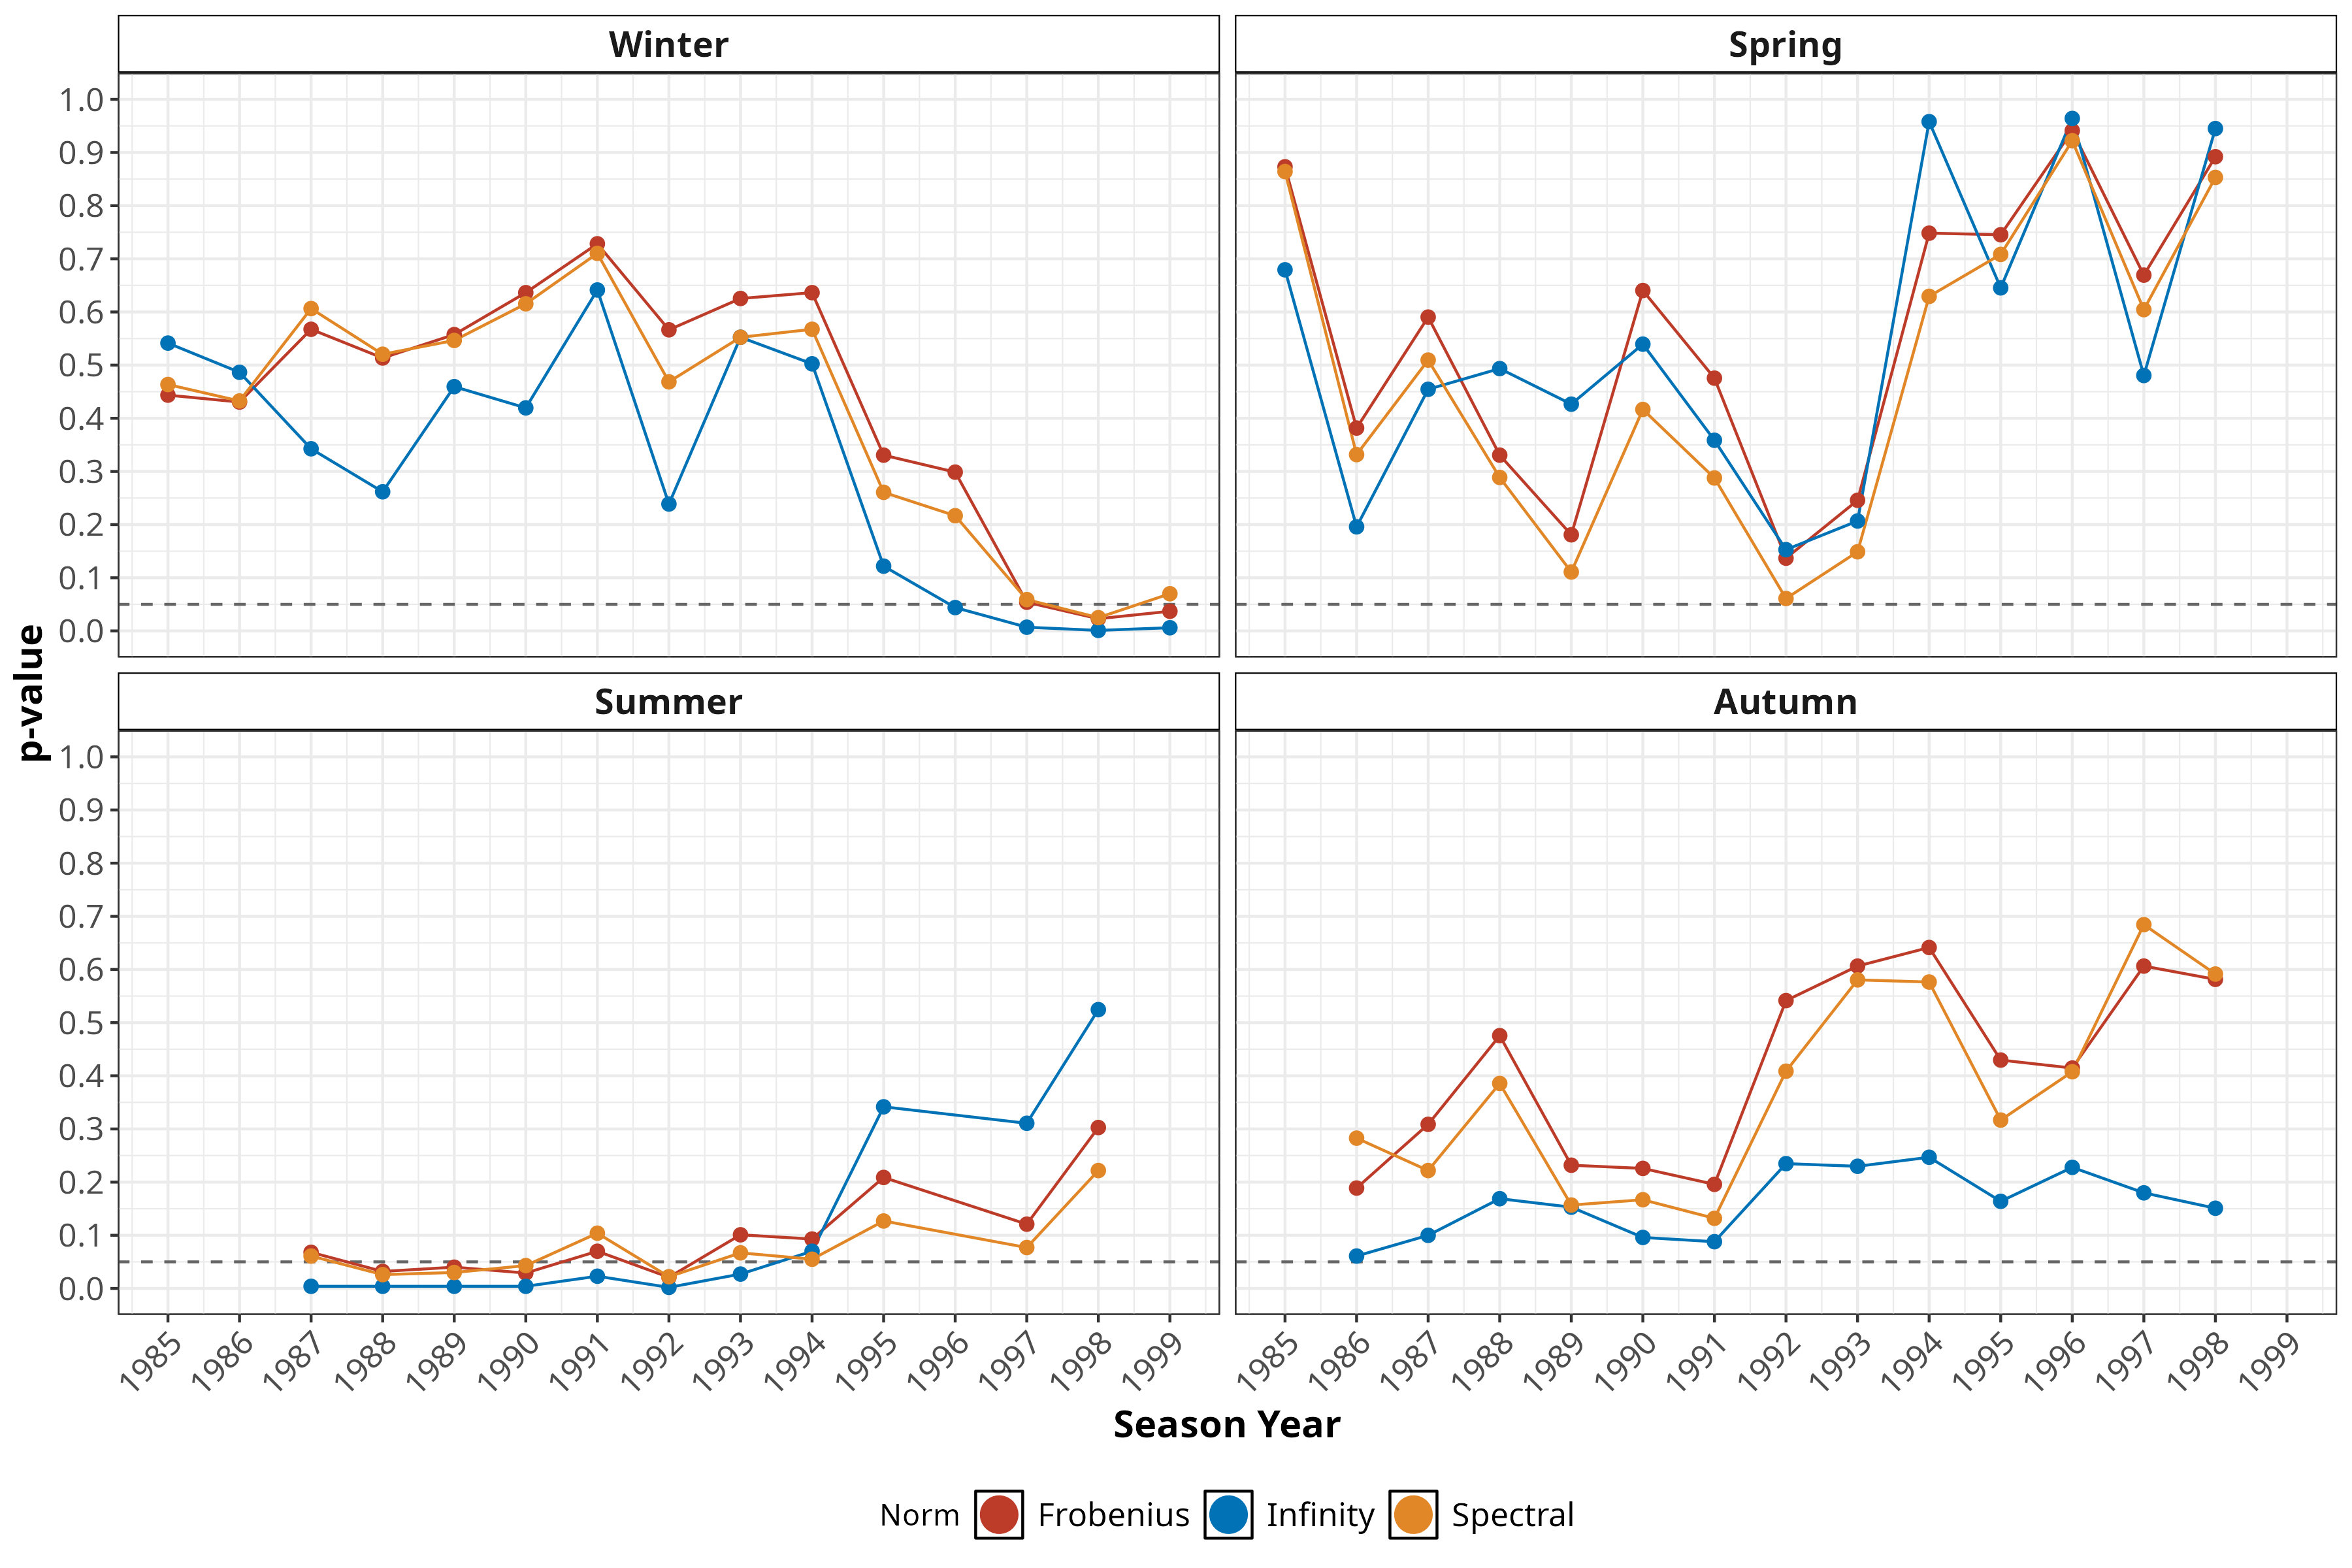
\includegraphics[width=0.9\linewidth]{plots/change.png}
\caption{
Pointwise permutation-test p-values for candidate changes in the seasonal extremal dependence structure, calculated using 25 season-years per temporal block and 200 permutations at each candidate. 
Results are shown for the Frobenius, infinity and spectral norms. 
A candidate $(t)$ represents a possible change between season-years $(t)$ and $(t+1)$. 
The horizontal dashed line denotes the pointwise 5\% significance level. 
}
\label{fig:app_cp}
\end{figure}


\subsection{Clustering Results}\label{subsec:app_clust}

% \begin{itemize}
%   \item We now fit the CE model one last time to the entire timeseries of Spring and Autumn data. 
%   \item For Summer, we fit the CE model separately for the season years 1960 to 1990 and 1990 to 2020, respectively, while for Winter, we do so for the season years 1960 to 1998 and 1999 to 2020. 
%   \item The resulting spatial clusterings from these fitted CE models is shown in Figure~\ref{fig:app_clust}. 
%   \item \todo{Comment on these results!!}
% \end{itemize}
% 
% \begin{figure}[htb]
%     \centering
%     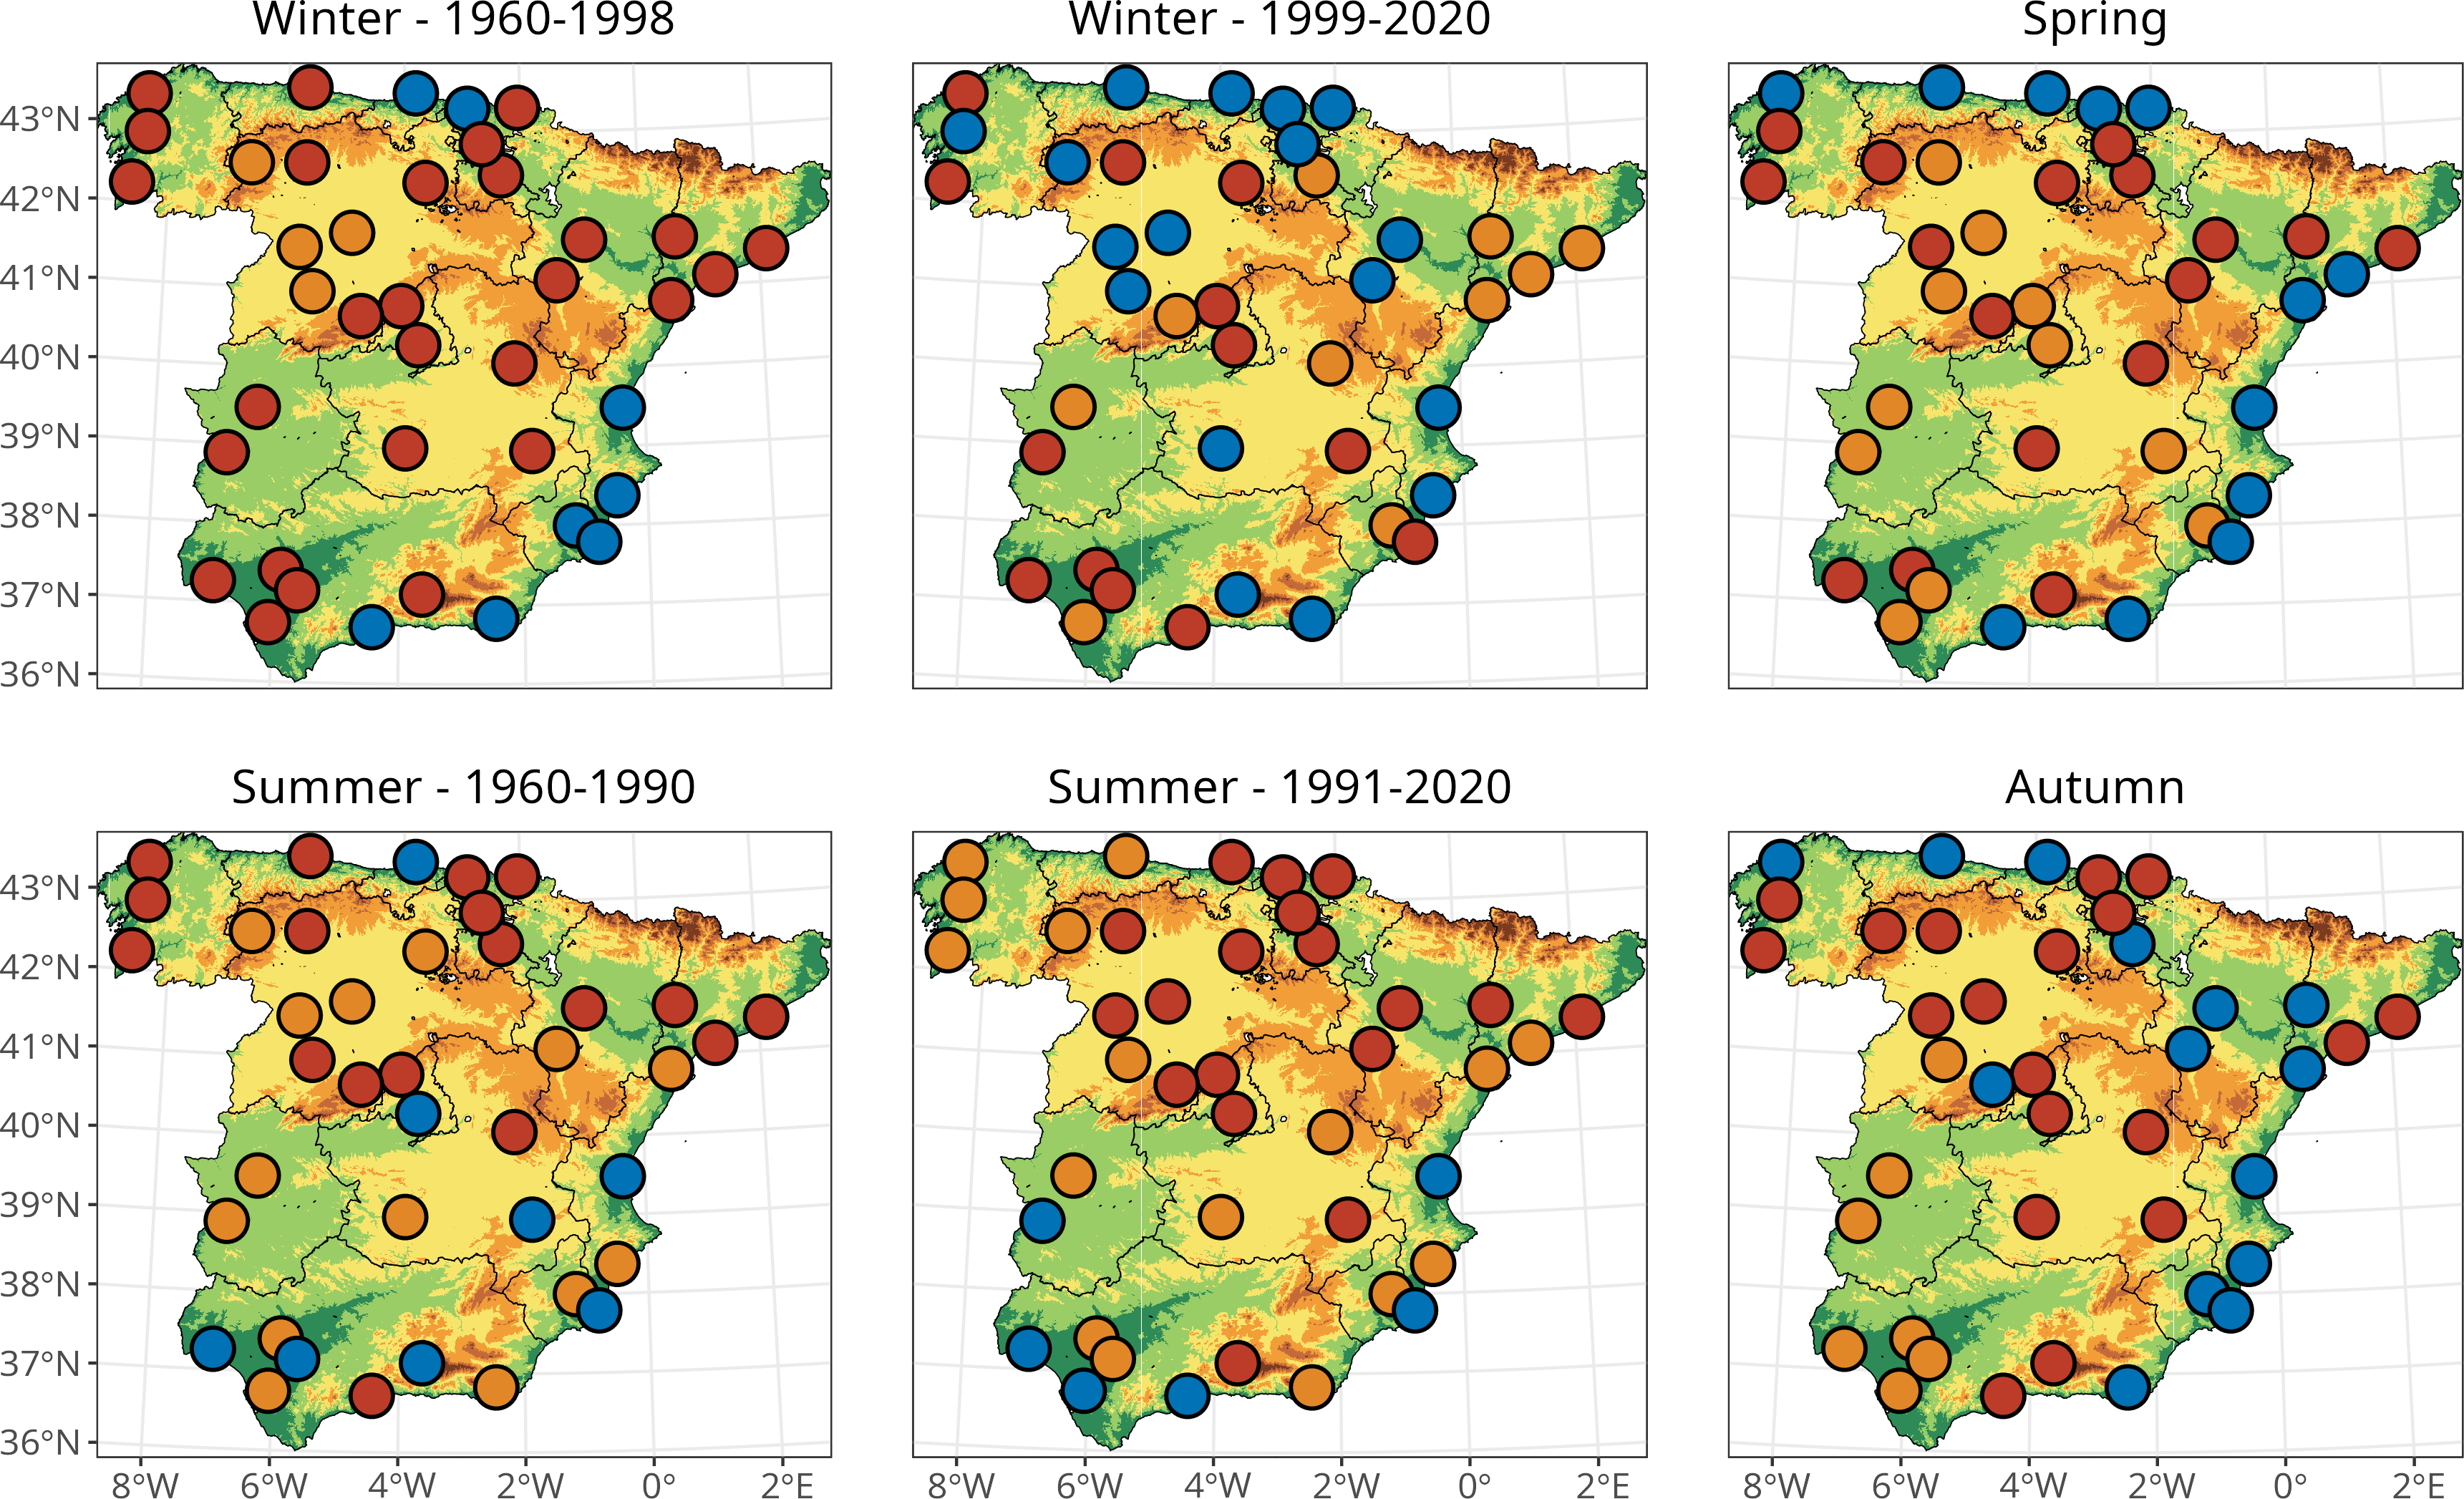
\includegraphics[width = 0.9\linewidth]{plots/clust_map_trim.png}
%     \caption{ 
%       Insert here
%     }
%    \label{fig:app_clust}
% \end{figure}

\begin{itemize}
\item We finally examine how the detected changes affect the spatial clustering of the fitted extremal dependence structure. 
\item For each fitted conditional extremes model, the aggregated dissimilarity matrix is used to partition the 40 stations into three clusters using the clustering procedure described in Section~\ref{sec:method}.
\item As the changepoint analysis provides no consistent evidence of a change in spring or autumn, we refit the conditional extremes model to the complete time series for these seasons. 

\item For summer, the pointwise tests identify a broader candidate change region during the late 1980s and early 1990s. 
\item We use 1990 as a representative division within this region and fit separate models to season-years 1960--1990 and 1991--2020.

\item For winter, the three norms provide their clearest common evidence at season-year 1998. 
\item We therefore fit separate models to winter season-years 1960--1998 and 1999--2020.

\item These divisions treat a candidate (t) as a change between season-years $(t)$ and $(t+1)$. \textcolor{red}{Confirm or update the selected divisions after completing the multiplicity-adjusted changepoint analysis.}
\end{itemize}

\begin{itemize}
\item Figure~\ref{fig:app_clust} presents the resulting spatial clusterings. 
\item Although station coordinates and elevation do not directly determine the clustering assignments, the fitted clusters exhibit substantial spatial coherence. 
\item Neighbouring stations are frequently assigned to the same cluster, suggesting that the estimated extremal dependence structure contains a strong geographical component.

\item The spring clustering broadly separates groups of stations along the northern and Mediterranean coasts (in blue) from groups in the western (orange) and central interior (red). 
\item Nevertheless, the boundaries are not determined solely by physical proximity, with some geographically separated stations assigned to the same dependence cluster.

\item The autumn clustering exhibits a stronger broadly coastal--interior structure. 
% \item Several stations along the northern and eastern coasts are grouped together, similar to the spring clustering, while clusters containing central, western and southwestern stations form comparatively coherent regional groupings.
\item Several stations along the northern and eastern coasts are grouped together, similar to the spring clustering, while the other two clusters comprise locations in the west/south-west and elsewhere, respectively. 

\item For summer, the two fitted periods retain some common large-scale structure.
\item However, a number of stations change their clustering relationships after 1990, most visibly in northwestern Spain, along the southern coast and across parts of the western interior. 
\item The summer changepoint therefore corresponds to a reorganization of particular regional relationships rather than a complete replacement of the earlier clustering structure.

\item The winter clustering, in contrast, changes more extensively across the 1998 division. 
\item In particular, the post-1998 fit produces a different grouping of many stations along the northern coast, in the western and central interior, and along the Mediterranean coast. 
\item This broader spatial reorganisation, as opposed to the more localised changes seen in summer, is consistent with the late-1990s signal being identified by all three norms in the changepoint analysis.
\end{itemize}

\begin{figure}[htb]
\centering
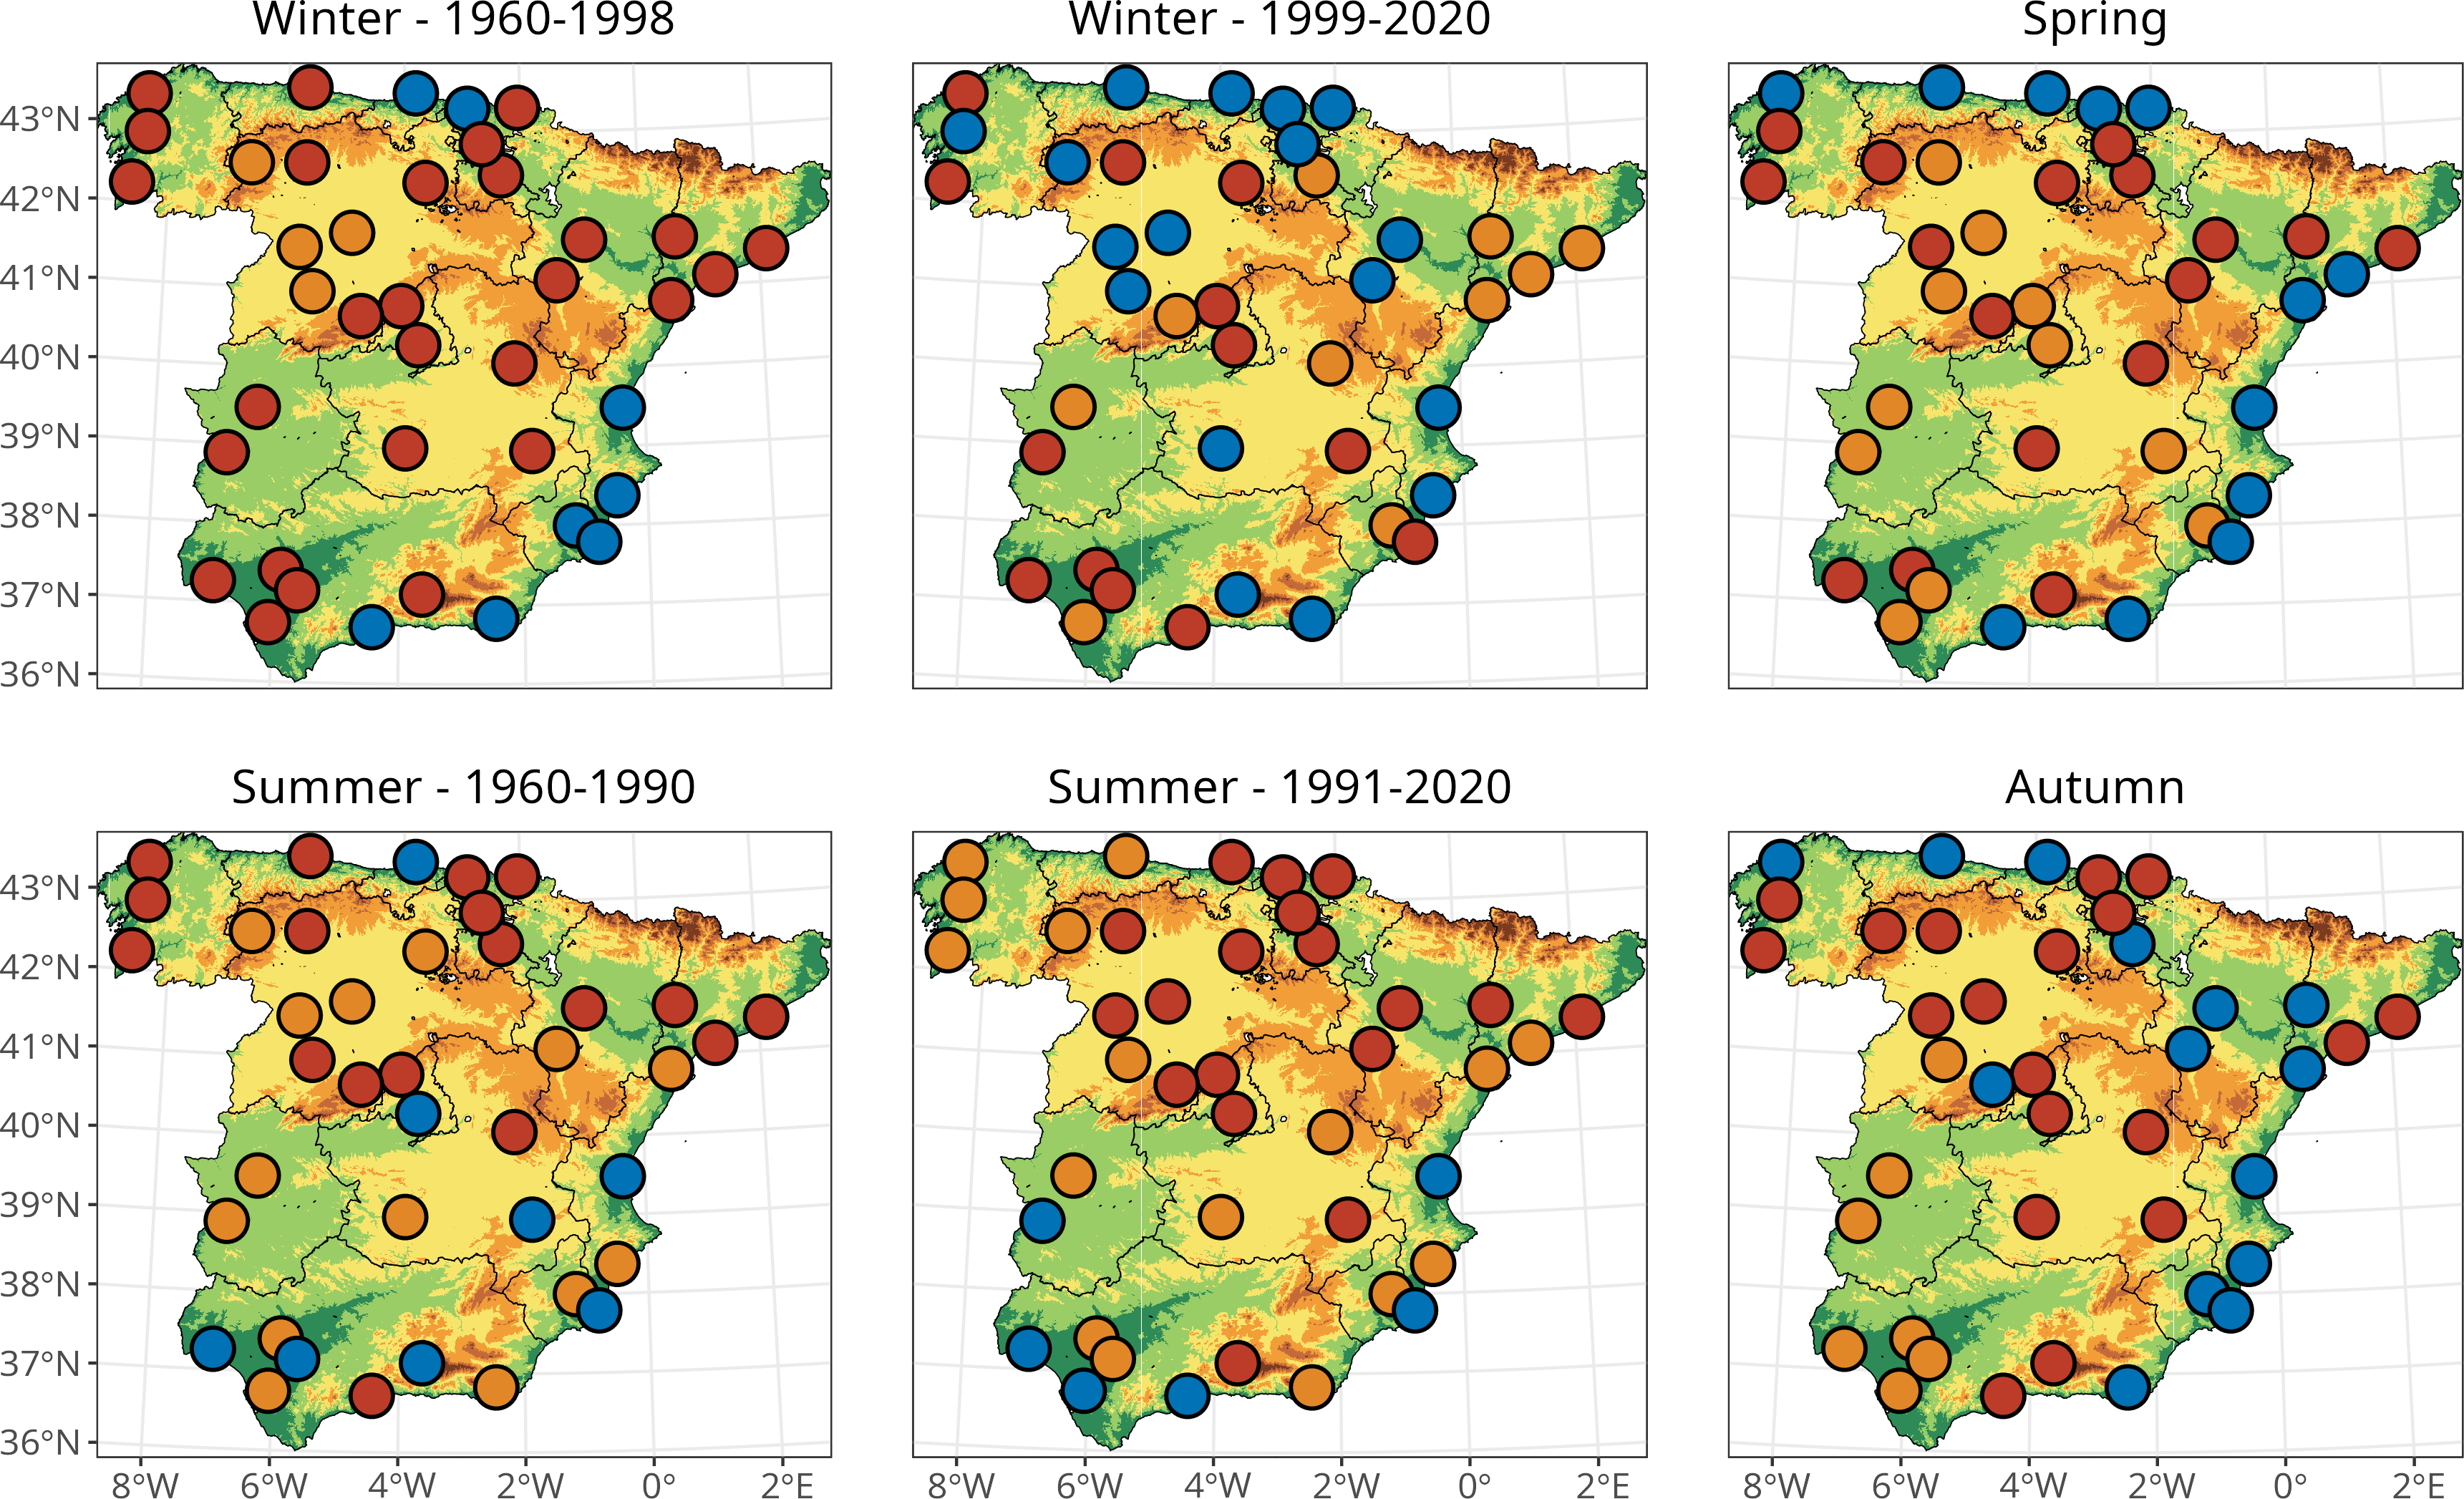
\includegraphics[width=0.9\linewidth]{plots/clust_map_trim.png}
\caption{
Spatial clustering of the 40 Spanish stations obtained from the fitted conditional extremes dissimilarity matrices. 
Spring and autumn are fitted using their complete time series. 
Summer is fitted separately for season-years 1960--1990 and 1991--2020, while winter is fitted separately for season-years 1960--1998 and 1999--2020. 
Three clusters are used in each fit. 
Colours distinguish cluster membership within each panel.
Background shading represents elevation.
}
\label{fig:app_clust}
\end{figure}


\section{Discussion}\label{sec5}

%\backmatter

\section*{Acknowledgments}
This is acknowledgment text~\cite{Elbaum2002}. Provide text here. This is acknowledgment text. Provide text here. This is acknowledgment text. Provide text here. This is acknowledgment text. Provide text here. This is acknowledgment text. Provide text here. This is acknowledgment text. Provide text here. This is acknowledgment text. Provide text here. This is acknowledgment text. Provide text here. This is acknowledgment text. Provide text here. 

\subsection*{Author contributions}

This is an author contribution text. This is an author contribution text. This is an author contribution text. This is an author contribution text. This is an author contribution text. 

\subsection*{Financial disclosure}

None reported.

\subsection*{Conflict of interest}

The authors declare no potential conflict of interests.


\section*{Supporting information}

The following supporting information is available as part of the online article:

% \noindent
% \textbf{Figure S1.}
% {500{\uns}hPa geopotential anomalies for GC2C calculated against the ERA Interim reanalysis. The period is 1989--2008.}
% 
% \noindent
% \textbf{Figure S2.}
% {The SST anomalies for GC2C calculated against the observations (OIsst).}


\appendix

\section{Section title of first appendix\label{app1}}

% \nocite{*}% Show all bib entries - both cited and uncited; comment this line to view only cited bib entries;
\bibliography{wileyNJD-APA}%


% \section*{Author Biography}
% 
% \begin{biography}{
\includegraphics[width=60pt,height=70pt,draft]{empty}}{\textbf{Author Name.} This is sample author biography text this is sample author biography text this is sample author biography text this is sample author biography text this is sample author biography text this is sample author biography text this is sample author biography text this is sample author biography text this is sample author biography text this is sample author biography text this is sample author biography text this is sample author biography text this is sample author biography text this is sample author biography text this is sample author biography text this is sample author biography text this is sample author biography text this is sample author biography text this is sample author biography text this is sample author biography text this is sample author biography text.}
% \end{biography}

\end{document}
